\chapter{Writing}
The essence of a document is the idea it represents. In the case of a text
document, this idea is articulated through speech, which is transcribed using
text, optionally accompanied by figures, and then laid out on a sheet of paper
according to a design. Since the text is typically independent on the design,
whose task is to support and elicit the internal structure of the text, it is
writing that is the logical first step in the text document creation.

\begin{figure}
  \input examples/01/trichter
  \caption{Exceptions that prove the rule about the separation of text and
    design can sometimes be encountered in poetry. Above is \person{Christian
    Morgenstern}'s \foreign[german]{\work{Trichter}}, where the text and its
    form are intimately intertwined.}
\end{figure}

The essentials of writing in any given natural language include \termpl*{grammar
rule}\index{writing rules!grammar}, which specify the structure of spoken
language, and \termpl*{orthographic rule}\index{writing rules!ortography}, which
impose additional requirements on written text. The complexity of either set of
rules depends entirely on the language in question. Some writing systems, such
as those that incorporate Chinese characters, are not phonographic and the
correspondence between the spoken words and the written symbols needs to be
memorized by the writer on a word-to-word basis. Other languages may use vastly
different grammar rules for speaking and for writing, which means that a spoken
sentence needs to be translated first before writing down. A writer needs to
recognize these specifics.

On top of grammar and orthographic rules stand \termpl{style guide}, which, in
order to improve consistency, codify how common language patterns are encoded.
More comprehensive style guides---such as \work{the Chicago Manual of Style} or
\work{the Oxford Style Manual}\sidenote{
  This document was prepared in accordance with \person{William Strunk}'s
  \work{Elements of Style}, an American English style guide for general use. 
}---often go beyond writing and provide guidelines on design and typesetting as
well, making them an indispensable reference on the editorial tradition.

Above all stand the \termpl*{typographic rule}\index{writing rules!typography},
which specify how the resulting document should be typeset so that it doesn't
disturb the eye of the reader. These, as well as the orthographic rules on
hyphenation, can be left out of consideration during writing, as it is the page
that should be formed around the writing and not the other way around.

\section{Text Processing}
Originally the domain of the pen, the quill, the stylus, and the more recent
typewriter machine, manuscripts of today are produced mainly using the personal
computer and stored in \termpl{text file}. The discipline of creating and
manipulating digital text is called \term{text processing} and will be the focus
of this section.

\subsection{Character Encoding}
Although computing at its most primal has no use for anything but numbers, it
has nevertheless been accompanied by text from the outset. Even the
earliest computers from 1950s were programmed with both raw machine code and
the text programming language of \acronym{FORTRAN}. The digital representation
of letters, digits and other characters was initially closely tied\sidenote{
  \Acronym{EBCDIC} by \acronym{IBM} was the default encoding on
  \acroshort{IBM}'s System/\kern-.4pt360 mainframes and was in active use until
  the introduction of \acronym{PC} in 1981. In writing systems using Chinese
  characters, special encodings, such as Big5, \acronym{JIS}, and \acronym{EUC},
  are used to this day. For brevity, the text focuses on the main stream of
  international encodings.}
to each specific application and processor architecture, but with the advent of
computer networking in 1960s, mutual intelligibility became a point of concern.
\quote{We had over sixty different ways to represent characters in
computers. It was a real Tower of Babel,} explains \person{Bob
Berner}~\cite{brandel99}, an American computer scientist who worked at
\acronym{IBM} during 1956--1962 and who drafted \acronym{ASCII}---a
\term{character encoding} from \citeyear{asa63} that unified the digital
representation of text across the computer industry and enabled computer
networking on a large scale.

\subsubsection{ASCII}
In \acronym{ASCII}, every character is represented by a number from zero to 127,
which is transformed to a seven-bit integer called a \term{character code}.
These 128 codes are used to encode \termpl{printable character}---spanning the
letters of the English alphabet, digits, punctuation, and other symbols---and
\termpl{control code}, as depicted in Table \ref{tab:ascii}.  Unlike printable
characters, control codes have no fixed visual representation and they were used
to implement application-specific communication protocols and text formatting;
their precise semantics were defined in a much later standard from
\citeyear{iso72}~\cite{iso72}. Unconstrained by the bandwidth and the storage
limitations of the 1960s and 1970s, today's communication protocols and text
formats gravitate towards markup constructed from printable characters, which,
unlike control codes, are easy to read and write by humans.

\begin{table}
  \input examples/01/ascii
  \caption{The \acronym{ASCII} encoding, as specified in the \citeyear{asa86}
    revision of the standard.~\cite{asa86}}
  \label{tab:ascii}
\end{table}

\begin{table}
  \input examples/01/utf8
  \caption{The \acroshort{UTF}-8 encoding. Each \textvisiblespace\ represents
    one bit of the \acroshort{UCS} code point in binary.}
  \label{tab:utf8}
\end{table}

\begin{table}
  \input examples/01/utf8-example
  \caption{An example of the \acroshort{UTF}-8 encoding}
  \label{tab:utf8-example}
\end{table}

%%% ASCII, Other Standards
%%%   <https://en.wikipedia.org/wiki/ASCII#Other_standards>
%%%   <https://en.wikipedia.org/wiki/ISO/IEC_8859-2#External_links>
%%%
%%% Character histories: notes on some Ascii code positions
%%%   <http://www.cs.tut.fi/~jkorpela/latin1/ascii-hist.html>
%%%
%%% ASCII: American Standard Code for Information Infiltration
%%%   <http://worldpowersystems.com/J/codes/>
%%%
%%% Encyclopedia of Computer Science, 4th edition
%%%   <https://dl.acm.org/ralston.cfm?CFID=698031209&CFTOKEN=46500462>
%%%
%%% Theoretical Foundation of Regular Expressions and Text Editors
%%%   <http://citeseerx.ist.psu.edu/viewdoc/download?rep=rep1&type=pdf&doi=10.1.1.126.9920>
%%%
%%% A History of Scientific Text Processing at CERN
%%%   <http://ref.web.cern.ch/ref/CERN/CNL/2001/001/tp_history/>
%%%
%%% When and how did text enter the world of computing, eventually to be
%%% standardized as ASCII in 1963? <http://qr.ae/RHFEzE>
%%%
%%% IBM's Early Computers: A Technical History
%%%   <http://www.amazon.com/IBMs-Early-Computers-Technical-Computing/dp/0262523930>

The following properties make it easy to manipulate and reason about character
strings encoded in \acronym{ASCII}:
\begin{itemize}
  \item Each character is represented by exactly seven bits. This makes it easy
    to allocate space for character strings of fixed length, to measure the
    number of characters stored in a memory region, and to perform basic
    operations, such as adjacent character retrieval or text truncation.
  \item Characters are alphabetically ordered. Character strings can therefore
    be collated by comparing character code binary values.
  \item Lowercase and uppercase letters, digits and control codes form
    contiguous ranges of character codes. This simplifies classification.
  \item There is precisely one way to encode any printable character. The
    conversion between the lower- and uppercase letters is a matter of
    inverting one bit.
\end{itemize}
This comes at the expense of support for non-English writing systems. As a
temporary workaround, a set of \acroshort{ASCII} derivatives that replaced the
less-needed characters of \# \$ @ [ \textbackslash\ ] \textasciicircum\ ` \{ |
\} and \textasciitilde\ for international characters was specified in the
\acroshort{ISO}~646 standard from \citeyear{iso72}.~\cite{iso72}

\subsubsection{Eight-bit Encodings}
With the byte size stabilizing at eight bits, new character encodings emerged
that were based on \acronym{ASCII} and used the additional bit to encode
characters of non-English writing systems while retaining complete backwards
compatibility with \acroshort{ASCII}. Beside the numerous vendor-specific
encodings (called \termpl{code page}), a set of fifteen eight-bit encodings
covering all major modern writing systems whose characters fit within the space
of 128 additional combinations was standardized in the
\acroshort{ISO}/\acroshort{IEC}~8859 series released during 1986--2001.

  % Show a time diagram of Czech encodings
  %   <http://luki.sdf-eu.org/txt/cs-encodings-faq.html>

Compared to \acronym{ASCII}, eight-bit encodings introduced an additional level
of complexity to text processing:
\begin{itemize}
  \item Each character is exactly eight bits wide. The manipulation with strings
    is therefore as straightforward as with \acronym{ASCII}.
  \item Character strings can no longer be collated by character code
    comparison. Each encoding requires separate collation tables.
  \item Classes of characters, such as uppercase and lowercase letters or
    punctuation, no longer form contiguous ranges and their position varies
    among encodings. This impedes character classification.
  \item Idiosyncrasies, such as the ligature of æ and invisible hyphenation
    hints, are included in several encodings, which makes it more difficult to
    determine character string equivalence. Algorithms for case conversion vary
    among encodings.
  \item There exists no standard mechanism to detect which encoding is being
    used. The distinction needs to be done on the application level using either
    heuristics, additional metadata, or human intervention. Consequently, no
    standard mechanism exists to use different character encodings within a
    single text document.
\end{itemize}
A portion of this complexity is inherent in the task of encoding the characters
of all modern writing systems, but the overhead caused by the character encoding
fragmentation proved to be unnecessary.

\subsubsection{The Universal Character Set and Unicode}\label{sec:ucs+unicode}
In the early 1990s, the continual increase in the available bandwidth and
storage led to the creation of the standards of
Unicode~\cite{unicode91,unicode92} and \acronym{UCS} in an attempt to create a
text encoding that would contain the characters of all the world's languages and
succeed \acronym{ASCII} as the \foreign[italian]{lingua franca} of text
interchange.

\Acronym{UCS} is an ever-expanding catalogue of characters from writing systems
both modern and ancient, and symbols ranging from diacritical marks,
punctuation, and ideograms to mahjong tiles, alchemical symbols, and the ancient
Greek musical notation. Each of these characters is assigned a number, called
a \term{code point}, ranging from 0 to 2,147,483,647 (\hexa{7FFFFFFF}) with the
numbers of the most common characters in the range from 0 to 65,535
(\hexa{FFFF}) called \acronym{BMP}. The smallest unit of division in
\acronym{UCS} are \termpl*{block}\acroindex[!block]{UCS}, which contain 256
thematically related characters. \Acronym{UCS} encodings map code points to
binary character codes and vise versa.

Three major encodings are specified in the \acronym{UCS} standard and its
amendments~\cite{iso93:am1,iso93:am2}:
\sidenote{%
  Notable are also the seven-bit encodings of \acroshort{UTF}-7
  \acroindex[!UTF-7@\acroshort{UTF}-7]{UTF} and \inx{Punycode}, which bring
  Unicode support to protocols that were designed with the seven-bit
  \acroshort{ASCII} in mind, such as e-mail.}
\begin{enumerate}
  \item[1]\acroshort{UTF}-32\acroindex[!UTF-32@{\acroshort{UTF}-32}]{UTF}
    directly encodes \acronym{UCS} characters by transforming their code points
    to four-byte integers. \acroshort{UTF}-32 is also known as
    \acroshort{UCS}-4\acroindex[!UCS-4@{\acroshort{UCS}-4}]{UCS}.
  \item[2]\acroshort{UTF}-16\acroindex[!UTF-16@{\acroshort{UTF}-16}]{UTF}
    directly encodes characters within \acronym{BMP} by transforming their code
    points to two-byte integers. Code points in the range from 65,536 to
    1,114,111 (\mbox{\hexa{010000}--\hexa{10FFFF}}) are transformed into pairs
    of two-byte integers, called \termpl{surrogate pair}, ranging from 55,296 to
    57,343 (\mbox{\hexa{DC00}--\hexa{DFFF}}). To enable the \acroshort{UTF}-16
    encoding, the code points in this range will never be assigned to
    characters~\cite[sec.\,3.4, D15]{unicode16}. The same is true of code points
    above 1,114,111 (\hexa{10FFFF}), which allows \acroshort{UTF}-16 to encode
    any \acroshort{UCS} character.
  \item[3]\acroshort{UTF}-8\acroindex[!UTF-8@{\acroshort{UTF}-8}]{UTF}
    directly transforms code points ranging from 0 to 127 (\hexa{7F}) to
    one-byte integers. Since the first \acroshort{UCS} block of the
    \acroshort{BMP} matches \acronym{ASCII}, any text encoded in eight-bit
    \acroshort{ASCII} is also encoded in \acroshort{UTF}-8. Code points in the
    range from 127 to 1,114,111 (\mbox{\hexa{00007F}--\hexa{10FFFF}}) are
    transformed into two to four one-byte integers ranging from 128 to 253
    (\mbox{\hexa{80}--\hexa{FD}}). The encoding is illustrated in tables
    \ref{tab:utf8} and \ref{tab:utf8-example}.
\end{enumerate}

\acroshort{UTF}-32 is primarily used for the fixed-space internal representation
of individual \acronym{UCS} characters inside programs, \acroshort{UTF}-16
fulfills a similar role in programs that only work with \acronym{BMP}, and
\acroshort{UTF}-8 is used for text storage and interchange. Since 2010, the
majority of text content on the Web has been encoded in \acroshort{ASCII} and
\acroshort{UTF}-8.~\cite{qsuccess15}

Unicode was a competing standard for universal text encoding that underwent a
merger with \acronym{UCS} in version 1.1 and since then, the standards have been
kept closely synchronised. Unicode is a superset of \acronym{UCS} which defines
additional information about \acronym{UCS} characters---such as their general
category, directionality, case, or numeric value~\cite[sec.\,3.5 and
ch.\,4]{unicode16}---, various text processing algorithms, and implementation
guidelines.

\begin{figure}
  \fsidenote{One of the design goals of \acroshort{UCS} was to avoid assigning
    code points to different glyphs that carry the same meaning. As a result,
    the visually distinctive Han characters used in the East Asian countries
    of China, Japan, Korea, and Vietnam were merged into a set of 75,960
    ideograms in a process referred to as the \term{Han Unification}
    \cite[sec.\,18.1]{unicode16}. This simplifies text processing, but also
    makes it impossible to encode a text in multiple East Asian languages
    without having to rely on external markup to select appropriate regional
    fonts. As a result, a derivative of \acronym{UCS} that doesn't implement the
    Han Unification was developed for use in operating systems based on
    \acronym{TRON} and is used in the East Asia alongside \acronym{UCS} and
    region-specific encodings.}
  \input examples/01/unihan
  \caption{Several Han characters in the traditional Chinese, Japanese,
    Korean, and Vietnamese variants}
\end{figure}

Regarding text processing, Unicode and \acronym{UCS} represent a compromise
between the simplicity of the seven-bit \acronym{ASCII} and the heterogeneity of
eight-bit encodings:
\begin{itemize}
  \item If simple text manipulation is preferred over space efficiency, each
    character can be made exactly two or four bytes wide using the
    \acroshort{UTF}-16 and \acroshort{UTF}-32 encodings.
  \item Although character strings can not be collated by a simple character
    code comparison, a collation algorithm is defined in the Unicode
    specification~\cite{unicode16:collation} and collation tables for major
    locales~\cite{unicode16:cldr} are maintained by the Unicode Consortium.
  \item Classes of characters---such as uppercase letters, lowercase letters,
    numbers, and punctuation---do not form contiguous ranges, but their position
    is directly specified in the standard~\cite[sec.\,4.5]{unicode16}.
  \item Although idiosyncrasies---such as ligatures, invisible hyphenation
    hints, and combining characters---are present in \acronym{UCS}, explicit
    normalization algorithms for character string equivalence testing are
    specified by the standard~\cite[sec.\,2.12]{unicode16}. An algorithm
    for case conversion is also specified~\cite[sec.\,3.13]{unicode16}.
    \index{Unicode!normalization}\index{Unicode!case conversion}
  \item The \ucs[FEFF]{Byte Order Mark} character can be inserted at the
    beginning of a text as a signature of Unicode encodings. As the name
    suggests, the order in which the \hexa{FE} and \hexa{FF} bytes arrive also
    indicates the order of bytes (called \term{endianity}) that was used to
    encode integers. In \acroshort{UTF}-32 and \acroshort{UTF}-16, endianity
    can be chosen arbitrarily by the encoding application. In \acroshort{UTF}-8,
    one-byte integers are used and the notion of endianity is therefore
    meaningless.
\end{itemize}

\begin{figure}
  \input examples/01/combining-chars
  \caption{Some \acroshort{UCS} characters can be either input as a single
    entity or composed from several combining characters. Regarding Unicode
    normalization forms, all of the above representations are canonically
    equivalent.}
\end{figure}

\begin{figure}
  \centerline{\code[sh]{iconv -f latin2 -t utf8 -- old.txt > new.txt}}%
  \caption{Text files can be converted between encodings using the
    \cliutil{iconv} command-line tool. The sample code shows the file
    \filename{old.txt} being converted from the
    \acroshort{ISO}/\acroshort{IEC}~8859-2 encoding to \mbox{\acroshort{UTF}-8}.
    The result of the conversion is stored in the file \filename{new.txt}.}
\end{figure}

%%% Setting collation order in shell sort
%%%   <http://superuser.com/a/414408/136765>
%%%
%%% Unicode 101: An Introduction to the Unicode Standard
%%%   <http://www.interproinc.com/blog/unicode-101-introduction-unicode-standard>
%%%
%%% Unicode Implementation levels
%%%   <http://www.cl.cam.ac.uk/~mgk25/unicode.html#levels>
%%%
%%% Unification of the Unicode Standard and ISO 10646
%%%   <http://www.unicode.org/versions/Unicode1.0.0/V2ch01.pdf>
%%%
%%% Unicode 88 <http://unicode.org/history/unicode88.pdf>
%%% Unicode equivalence <https://en.wikipedia.org/wiki/Unicode_equivalence>
%%%
%%% Plane (Unicode):
%%%   <https://en.wikipedia.org/wiki/Plane_(Unicode)#Basic_Multilingual_Plane>

\begin{figure}[p]
  \centerline{\includegraphics[width=0.75\textwidth]%
    {examples/01/google-pinyin.png}}
  \caption{Text input methods are not limited to keyboard layouts. Software that
    enables the input of non-Latin characters on a keyboard through reversed
    romanization can often be the best option for writing systems with a large
    number of characters. Above is the \inx{Google Pinyin} input method for the
    Android operating system, which makes it possible to input Chinese
    characters using the \inx{pinyin} phonetic system.}
\end{figure}

\begin{figure}[p]
  \input examples/01/composeKey
  \caption{The \key{Compose}\index{Compose key@\displaykey{Compose} key} key
    followed by a mnemonic sequence of \acroshort{ASCII} characters produces a
    \acroshort{UCS} character. Although originally a physical key, \key{Compose}
    is not available on modern \acroshort{PC} and Apple keyboards and is usually
    mapped to the right \key{Ctrl} or \key{Super} key in software.
    \key{Compose} is natively supported on \Unices\ using the \inx{X Window
    System}. On other operating systems, support can be added by third-party
    software.}
\end{figure}

\begin{figure}
  \input examples/01/altCodes
  \caption{On the Windows operating system, holding the \key{Alt} key and typing
    a sequence of numbers produces a character with the corresponding number
    from either an \acroshort{IBM} code page, if the number has no leading zero,
    or from a Windows code page otherwise. The code pages vary depending on the
    current locale; in English locales, the \acroshort{IBM} code page~437
    and the Windows code page~1252 are used. After a Windows Registry
    modification, it is also possible to directly produce \acroshort{UCS}
    characters by holding the \key{Alt} key and typing the corresponding
    \acroshort{UCS} code point in hexadecimal.}
\end{figure}

\subsection{Text Input}
To insert text into a document, it is necessary to use an input device. In case
of personal computers, this is typically a computer keyboard and a mouse,
although the ongoing research in the areas of \acronym{SR} and \acronym{OCR}
makes it possible to use a microphone or a tablet as well. On hand-held devices,
the use of either a numeric keypad or a touch-screen is more typical.

An operating system will typically provide one or more input methods for each
input device through a component commonly referred to as the \acronym{IME}. The
\acroshort{ASCII} encoding was developed with typewriters and teleprinters in
mind and, as their direct descendant, the standard computer keyboard provides
support for all \acroshort{ASCII} characters. This doesn't apply to the much
larger \acronym{UCS} and it is the task of an \acronym{IME} to provide a
mechanism for the creation and selection of keyboard layouts that will allow the
user to input any \acronym{UCS} character. Some programs may provide input
methods of their own that are independent on the \acronym{IME}.

\subsection{Text Editors}
A \term{text editor} is an application that can be used to create and modify
text files. Entry-level text editors are often distributed with an operating
system and offer little beyond the ability to load, modify, and save text files
in a text encoding of choice. Entry-level text editors with a \acronym{GUI}
include the free \inx{Leafpad} for \Linux\ and \acronym{BSD} family of operating
systems, and the proprietary \inx{Notepad} for Windows and \inx{TextEdit} for
Mac OS. Entry-level text editors with a \acronym{CLI} include the free
\cliutil{joe}, \acroshort{GNU}
\cliutil*{nano}\acroindex[!nano@\cliutil*{nano}]{GNU}, and \cliutil{pico}.

More advanced text editors come with the support for \termpl{regular expression}
and \term{version control}---which will be covered in sections \ref{sec:regexs}
and \ref{sec:vcs}---and user modules that extend the base functionality.
Advanced \acronym{GUI} text editors include the free \inx{Notepad++} and
\inx{Atom}, and the proprietary \inx{Sublime Text}.  Advanced \acronym{CLI} text
editors include the free \inx{Emacs}, \cliutil{vi}, and \cliutil{vim}. These
\acronym{CLI} text editors are notorious for their steep learning curve; in
exchange, they empower the users to perform complex text editing.

\subsection{Interactive Document Preparation Systems}
Interactive \acropl{DPS}\acroindex[!interactive]{DPS} are a breed of text
editors that produces fully formatted text documents instead of (or along with)
text files. The reader is advices to avoid interactive \acropl{DPS} that use
proprietary, undocumented, or obscure file formats which lock the user into
using the respective \acronym{DPS}. Well-defined interactive \acronym{DPS} file
formats include \acronym{PDF}, \acronym{OOXML}, and \acronym{ODF}.

The primary difference between text editors and \acropl{DPS} is the fact that
the user is expected to use the \acronym{DPS} to mark up, design, and typeset the
resulting text document, whereas with plain text files a multitude of choices is
available at each step of the document preparation process. The self-sufficient
nature of \acropl{DPS} may be a time-saving feature for simpler documents, but
in the case of more complex documents, the markup and typesetting capabilities
of a \acronym{DPS} may not be up to par with those of a dedicated tool.
Interactive \acropl{DPS} include the free \inx{Apache OpenOffice} and
\inx{Scribus}, and the proprietary \inx{TextEdit}, \inx{Microsoft Word},
\inx{Scribus}, \inx{Adobe InDesign}, \inx{Adobe FrameMaker}, and
\inx{QuarkXPress}.

\subsection{Regular Expressions}\label{sec:regexs}
The \term{Chomsky hierarchy}\index{Noam Chomsky!hierarchy} is a classification
of text production rule sets (called \termpl{formal grammar}), which was
proposed~\cite{chomsky56} in \citeyear{chomsky56} by the American linguist
\person{Noam Chomsky} in his endeavor to discover a good formal model for the
description of natural languages. The class of \termpl{regular grammar}, which
is the least powerful of the proposed classes, and the related formal model of
\termpl{regular expression} enable the writer to match patterns within text.

Since regular expressions are just a formal model, a software implementation
needs to settle on a concrete syntax. One of the earliest standard syntaxes are
\acronym{BRE} and \acronym{ERE} syntaxes~\cite[part~1,~ch.\,9]{iso93:posix2}
described in Table \ref{tab:regexs}, which are supported by most text processing
programs on \Unices.

More extensive syntaxes include the \acroshort{GNU} extensions of \acronym{BRE}
and \acronym{ERE}, the regex syntax of the \inx{Perl} programming language, and
their derivatives. For these syntaxes, the term \term*{regular} is a misnomer,
as they can be used to describe formal grammars that, according to the Chomsky
hierarchy, are stronger than regular.\sidenote{
  \citework{friedl06} by \person{Jeffrey E. F. Friedl} is an extensive resource
  on regexes.}
To disambiguate the term, expressions in these syntaxes are often called
\termpl*[regexes]{regex}\index[see{regular expression}]{regex}.

\begin{table}
  \input examples/01/regexs
  \label{tab:regexs}
\end{table}

%%% POSIX.2-1997: Regular Expressions
%%%   <http://pubs.opengroup.org/onlinepubs/007908799/xbd/re.html>

Many regex syntaxes and the software that implements them were designed for the
processing of \acronym{ASCII} text and may behave in surprising ways, when
confronted with \acronym{UCS} characters. The software may assume that each
character is exactly one byte wide and fail to recognize any character that
occupies several bytes. It may also assume that all \acronym{UCS} characters
fall within \acronym{BMP} and exhibit the same problem with characters outside
\acronym{BMP}. More subtle, but no less precarious, can be the lack of support
for Unicode case conversion and normalization algorithms, which makes it
difficult to perform robust case-insensitive matching and the matching of
characters that can be encoded in several different ways. The lack of awareness
of the invisible characters that can appear in \acronym{UCS} text---such as the
\ucs[200B]{zero width space}, \ucs[200C]{zero width non-joiner}, \ucs[200D]{zero
width joiner}, and \ucs[FEFF]{zero width no-break space}---, is also problematic
and can lead to false negative matches. Conversely, modern regex syntaxes that
at least partially implement the Unicode standard for Regular
Expressions~\cite{unicode13}---such as those of Perl 5.2 or Java 7---are
actively aware of \acronym{UCS} and provide features that enable the matching of
characters based on their general category, numeric value, directionality, and
other properties defined by Unicode, as shown in Table \ref{tab:unicode-regexs}.

\begin{table}[!tb]
  \input examples/01/unicode-regexs
  \caption{The elements of the Unicode regex syntax implemented by Perl 5.2
    and Java 7. The list of properties is not exhaustive.}
  \label{tab:unicode-regexs}
\end{table}

The most elementary text processing \acroshort{CLI} program is \cliutil{grep}%
\sidenote{
  The authoritative resource on \cliutil{grep}, \cliutil{sed}, and \cliutil{awk}
  is \citework{dougherty97}, which explains each program as well as the
  \acroshort{BRE} and \acroshort{ERE} syntaxes in full detail.
}, which makes it possible to search text files for fixed strings and regexes in
default of an advanced text editor. Unless configured otherwise, the tool will
present lines that contain one or more matches to the user. A more advanced
text-processing \acroshort{CLI} program is \cliutil{sed}, which features a
simple programming language that can be used to arbitrarily search and transform
text files. \Cliutil{awk} is a \acroshort{CLI} program that also features a
text-processing programming language, albeit a more advanced one than that of
\cliutil{sed}. Originally developed for the Research Unix during 1973--1977,
\cliutil{grep}, \cliutil{sed}, and \cliutil{awk} are available in various
flavors for most operating systems.

%%% The true power of regular expressions
%%%   <https://nikic.github.io/2012/06/15/The-true-power-of-regular-expressions.html>
%%%
%%% Regular Expression Matching Can Be Simple And Fast
%%%   <https://swtch.com/~rsc/regexp/regexp1.html>
%%%
%%% JavaScript has a Unicode problem
%%%   <https://mathiasbynens.be/notes/javascript-unicode>

\section{Version Control}\label{sec:vcs}
When writing a text document, it is often useful to have a backup of the
previous versions of files, so that undesirable changes can be reverted whenever
necessary. If more than one person contributes to the document, the ability to
track the authorship of these changes also becomes an asset. At their most
rudimentary, \acronym{VCS} record changes along with their descriptions and
authorship information. These changes can then be viewed, and reverted.
With a single contributor, \acronym{VCS} are a convenient alternative to manual
version archival. With several contributors, \acronym{VCS} become an essential
tool.

\Acronym{VCS} can be dichotomized based on their architecture, which is either
\term*{centralized}\acroindex[!centralized]{VCS} or \term*{decentralized}
\acroindex[!decentralized]{VCS}. Centralized \acronym{VCS} store all versions
in a repository located on a remote server. Users send new versions to the
server and retrieve existing versions using a client software. The client
software is \term*{thin} in the sense that it does not store more than one
version locally and its operation is fully dependent on the availability of the
server. An example of centralized \acronym{VCS} is \acronym{SVN}\sidenote{%
	The authoritative resource on \acronym{SVN} is \citework{sussman02},
	affectionately known as \work{the Subversion book}.}.

By comparison, there is no designated server in decentralized \acronym{VCS} and
the users can upload and download new versions directly from one another. The
client software is \term*{thick} in the sense that all users have a local
repository with every existing version, which they can view and manipulate
at any time. The disadvantages include the more complex workflow, greater
storage size requirements and the increased opportunity for the users not to
share their local changes frequently enough, leading to an increased chance of
collisions. Examples of decentralized \acronym{VCS} include \inx{Git},
\inx{Mercurial}, or \inx{Bazaar}.

\begin{figure}
  \input examples/01/svn
  \caption{The basic \acroshort{SVN} workflow}
\end{figure}

\begin{figure}
%  \fsidenote{Although it is typical to use a central repository, the
%    decentralized architecture of Git makes it possible for clients to exchange
%    the contents of their repositories directly.  Multiple layers of
%    repositories that automatically exchange the latest updates can also be
%    created for backup and other purposes.}
  \input examples/01/git
  \separatorcaption{The diagram above depicts the basic Git workflow. The
    diagram below depicts the use of the Git program with an \acroshort{SVN}
    repository; this bears all the advantages and disadvantages associated with
    decentralized \acronym{VCS}.}
  \input examples/01/git-svn
\end{figure}

Although \acronym{VCS} can be used to keep track of any kind of files, they are
especially geared towards text files, which they can easily display along with
changes. However, most interactive \acropl{DPS} do not produce text files, which
can make version control challenging. As a solution, some \acropl{DPS} include
internal version control functionality that can record changes directly into
output files. Other \acropl{DPS}\sidenote{%
  An example would be the graphical \acroshort{SVN} client \inx{Tortoise
  \acroshort{SVN}} that is able to display the changes between two versions
  of Microsoft Word documents using the interface provided by Microsoft Office.
} provide an interface for external \acronym{VCS} to display changes between two
versions of output documents produced by the \acropl{DPS}. A category of its own
form web services that enable real-time interactive collaboration---such as
\inx{Word Online} or \inx{Google Documents}.

\begin{figure}
  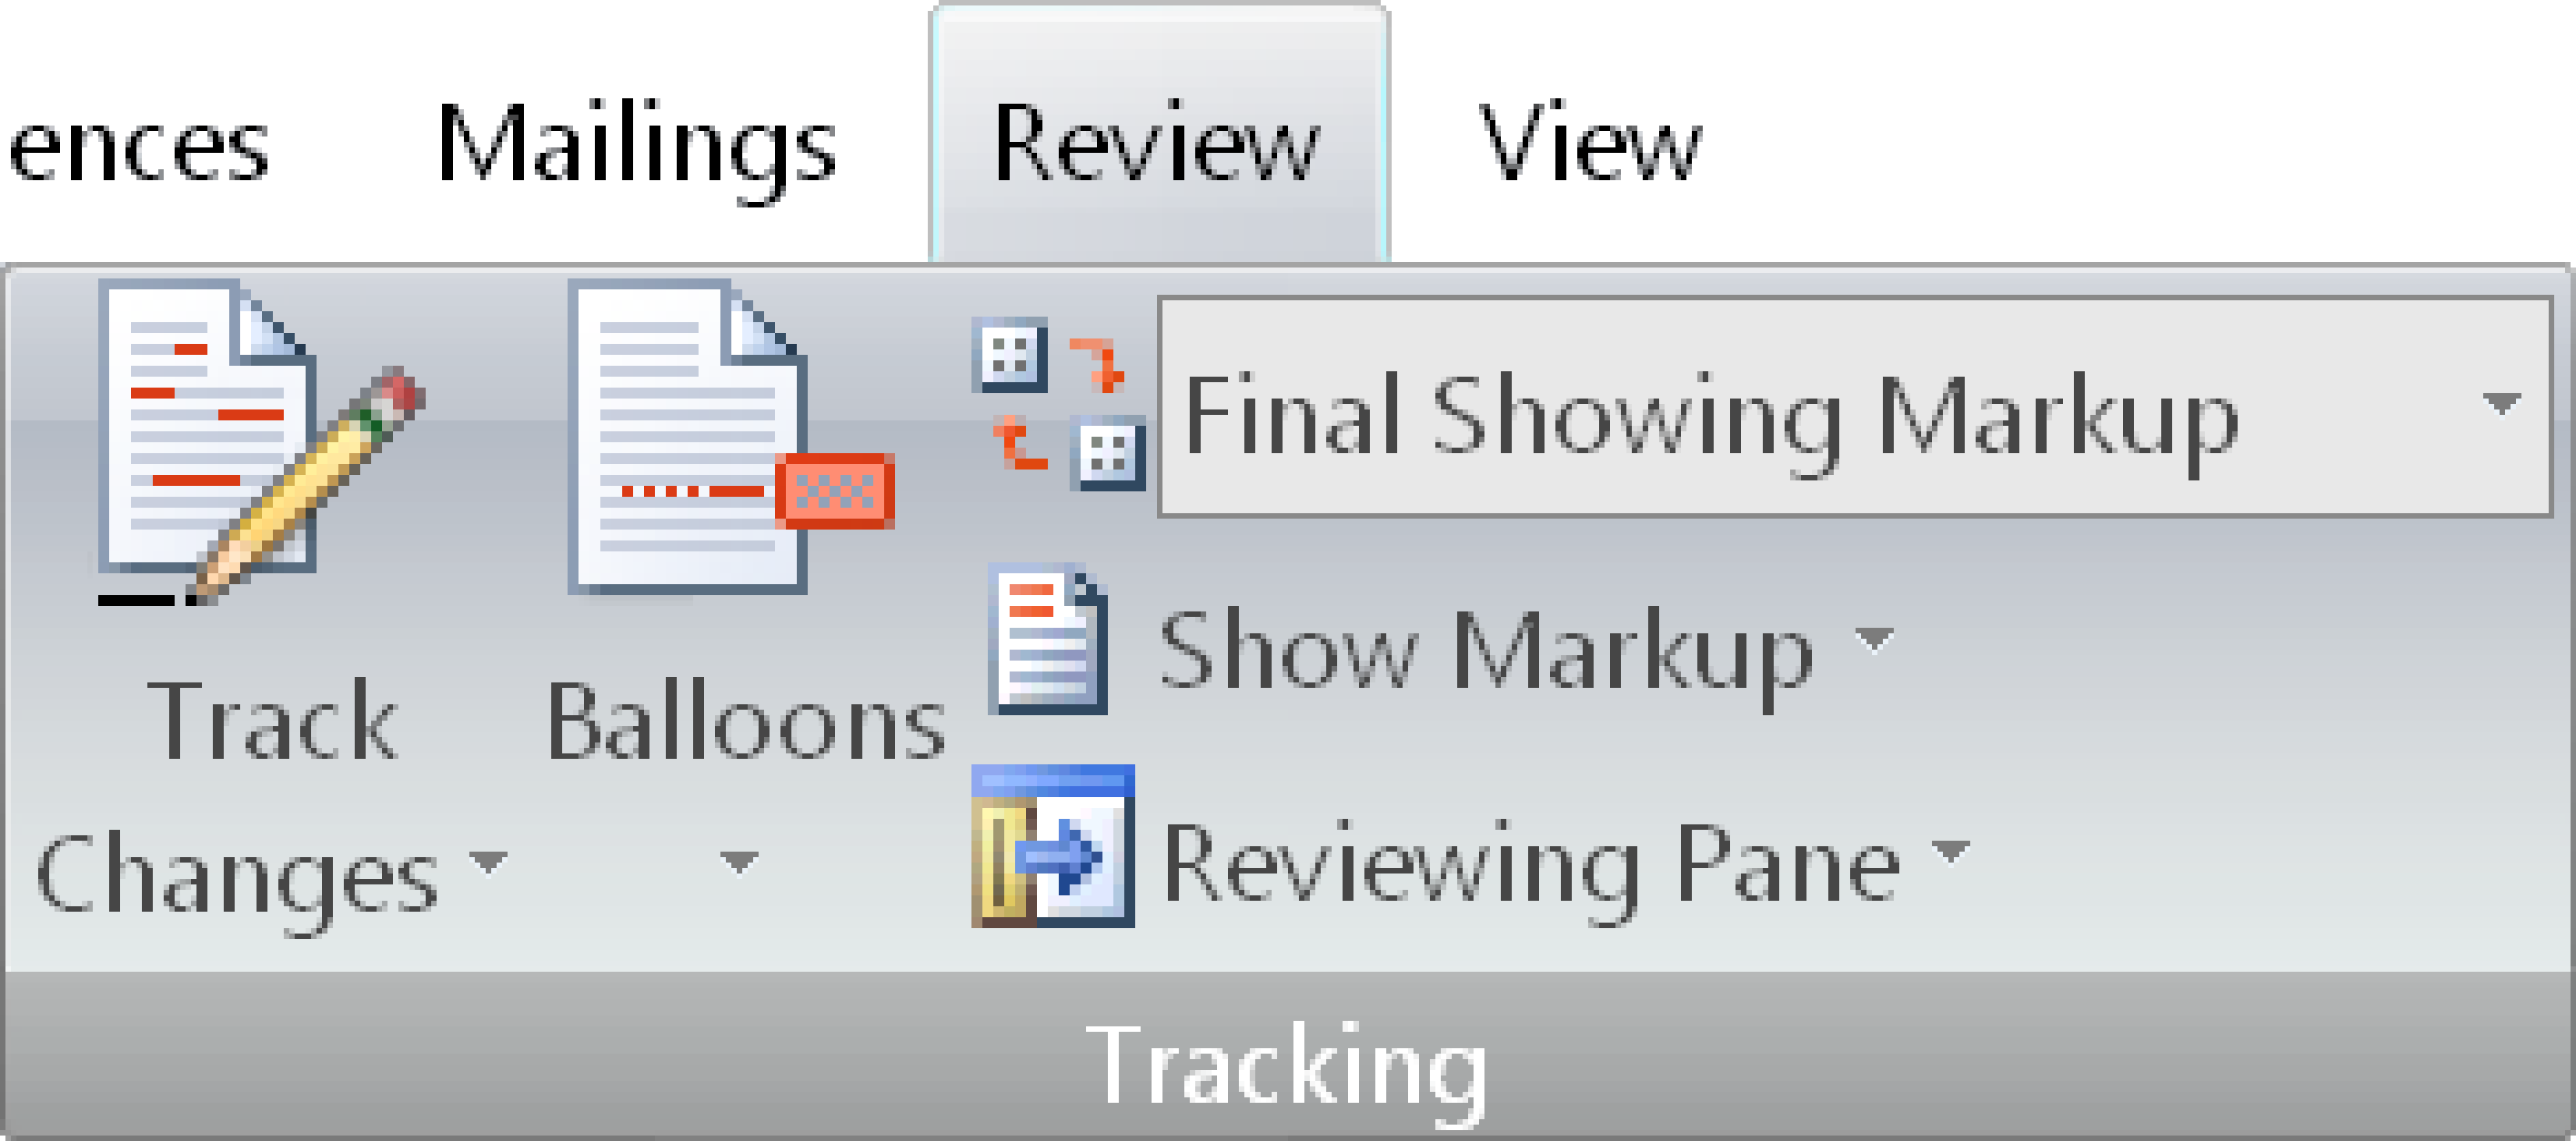
\includegraphics[width=\textwidth]{examples/01/word.png}\nextimage
  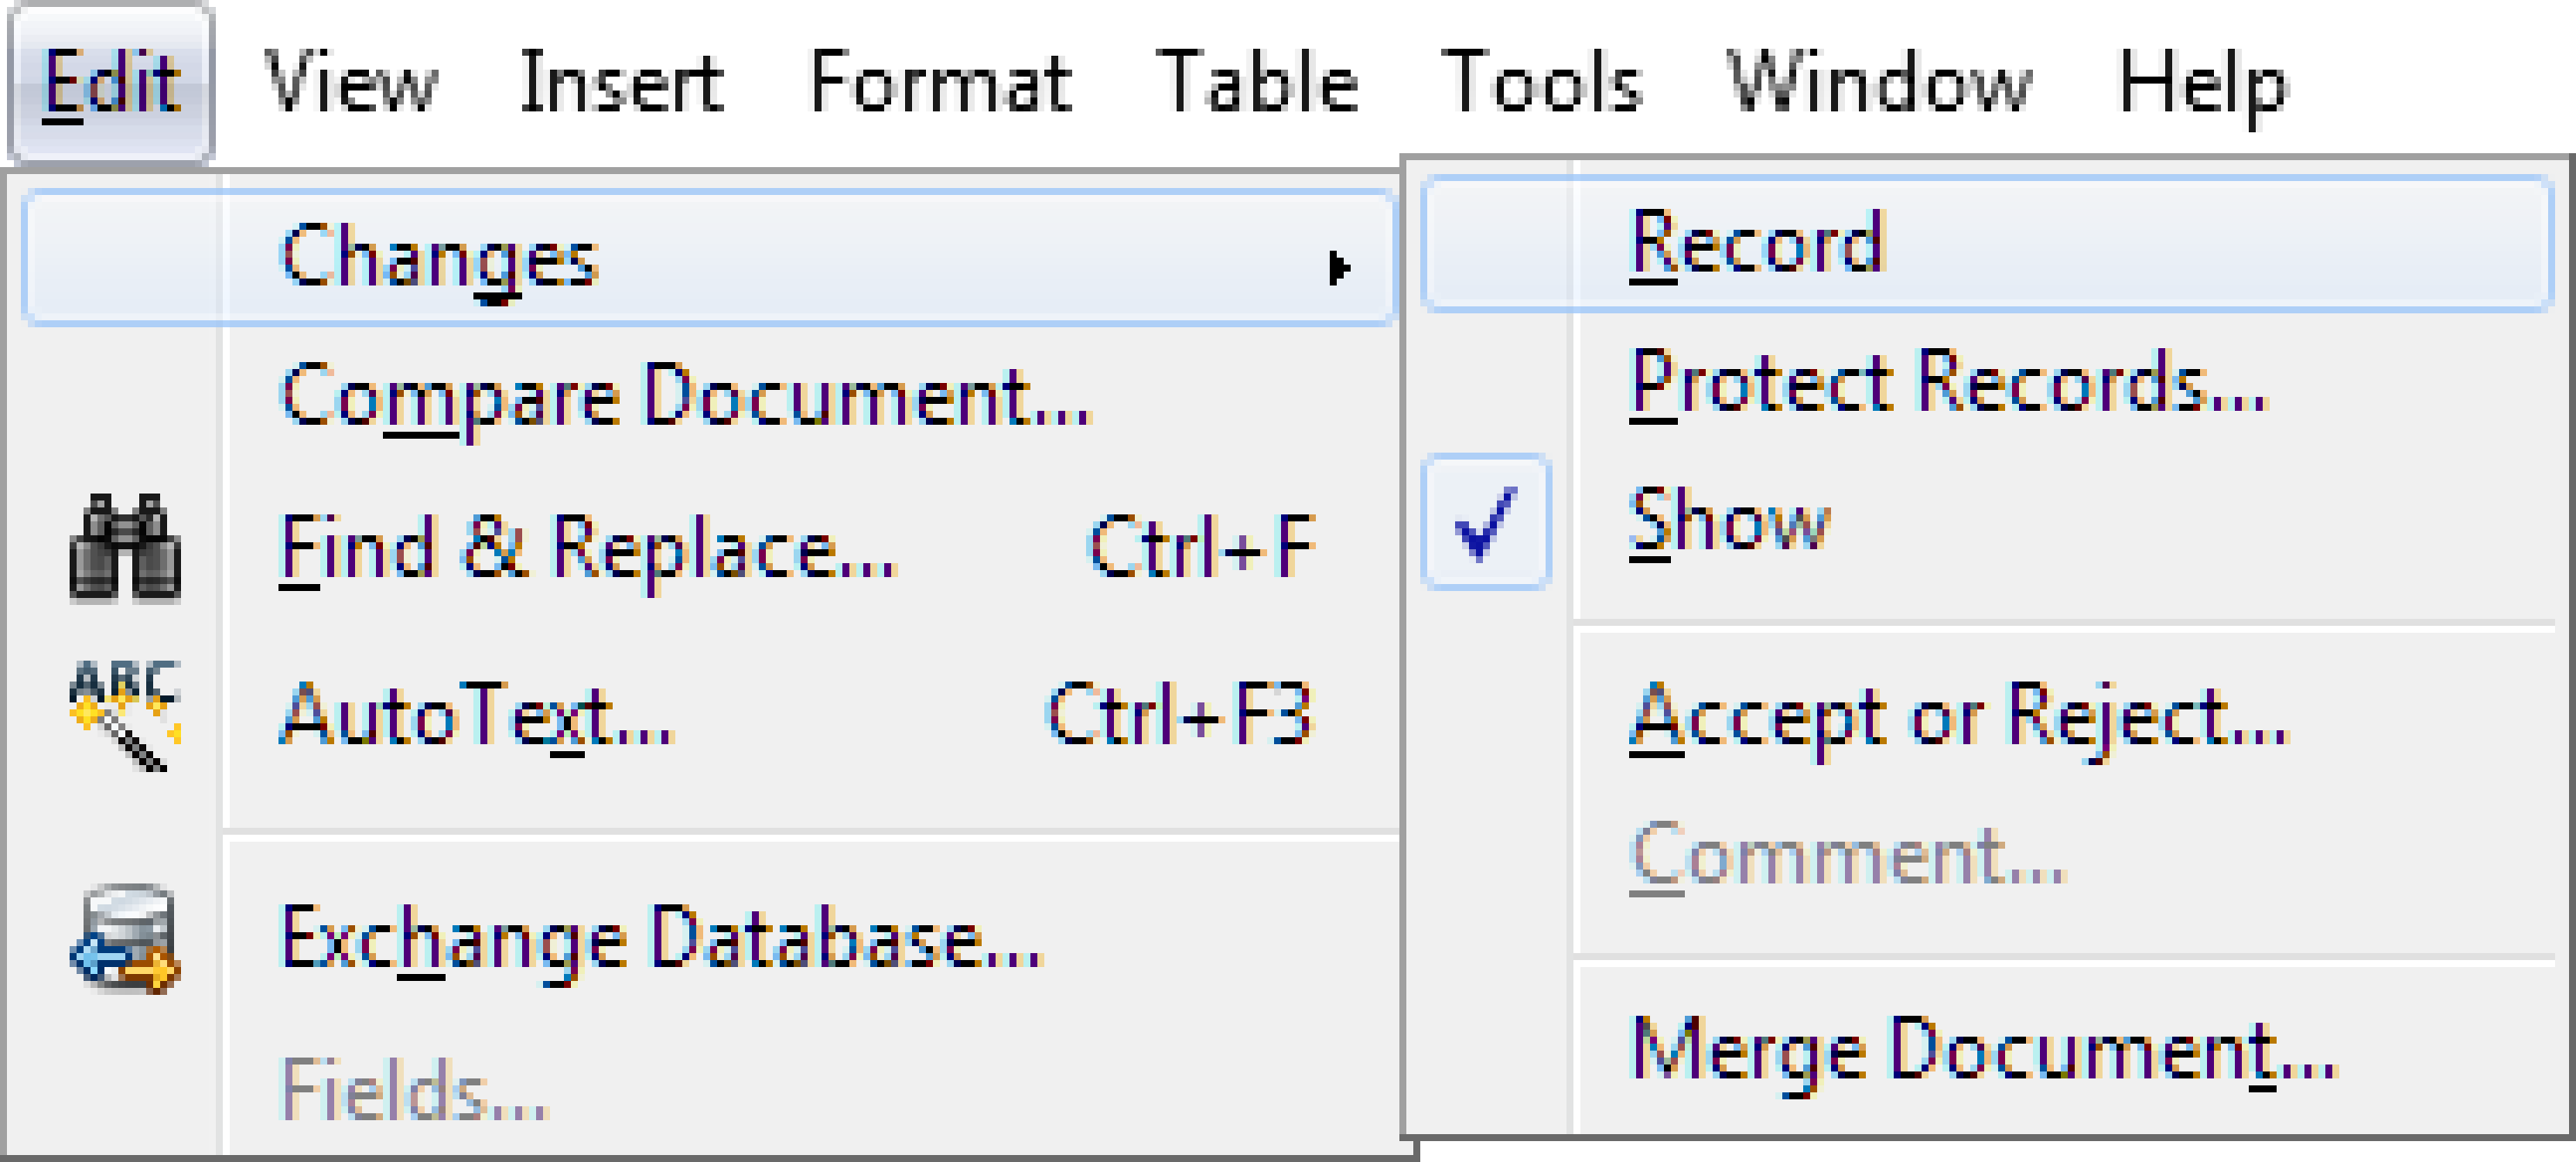
\includegraphics[width=\textwidth]{examples/01/openoffice.png}
  \separatorcaption{The built-in \acronym{VCS} of \inx{Microsoft Word} (top) and
    \inx{Apache OpenOffice} (bottom)}
  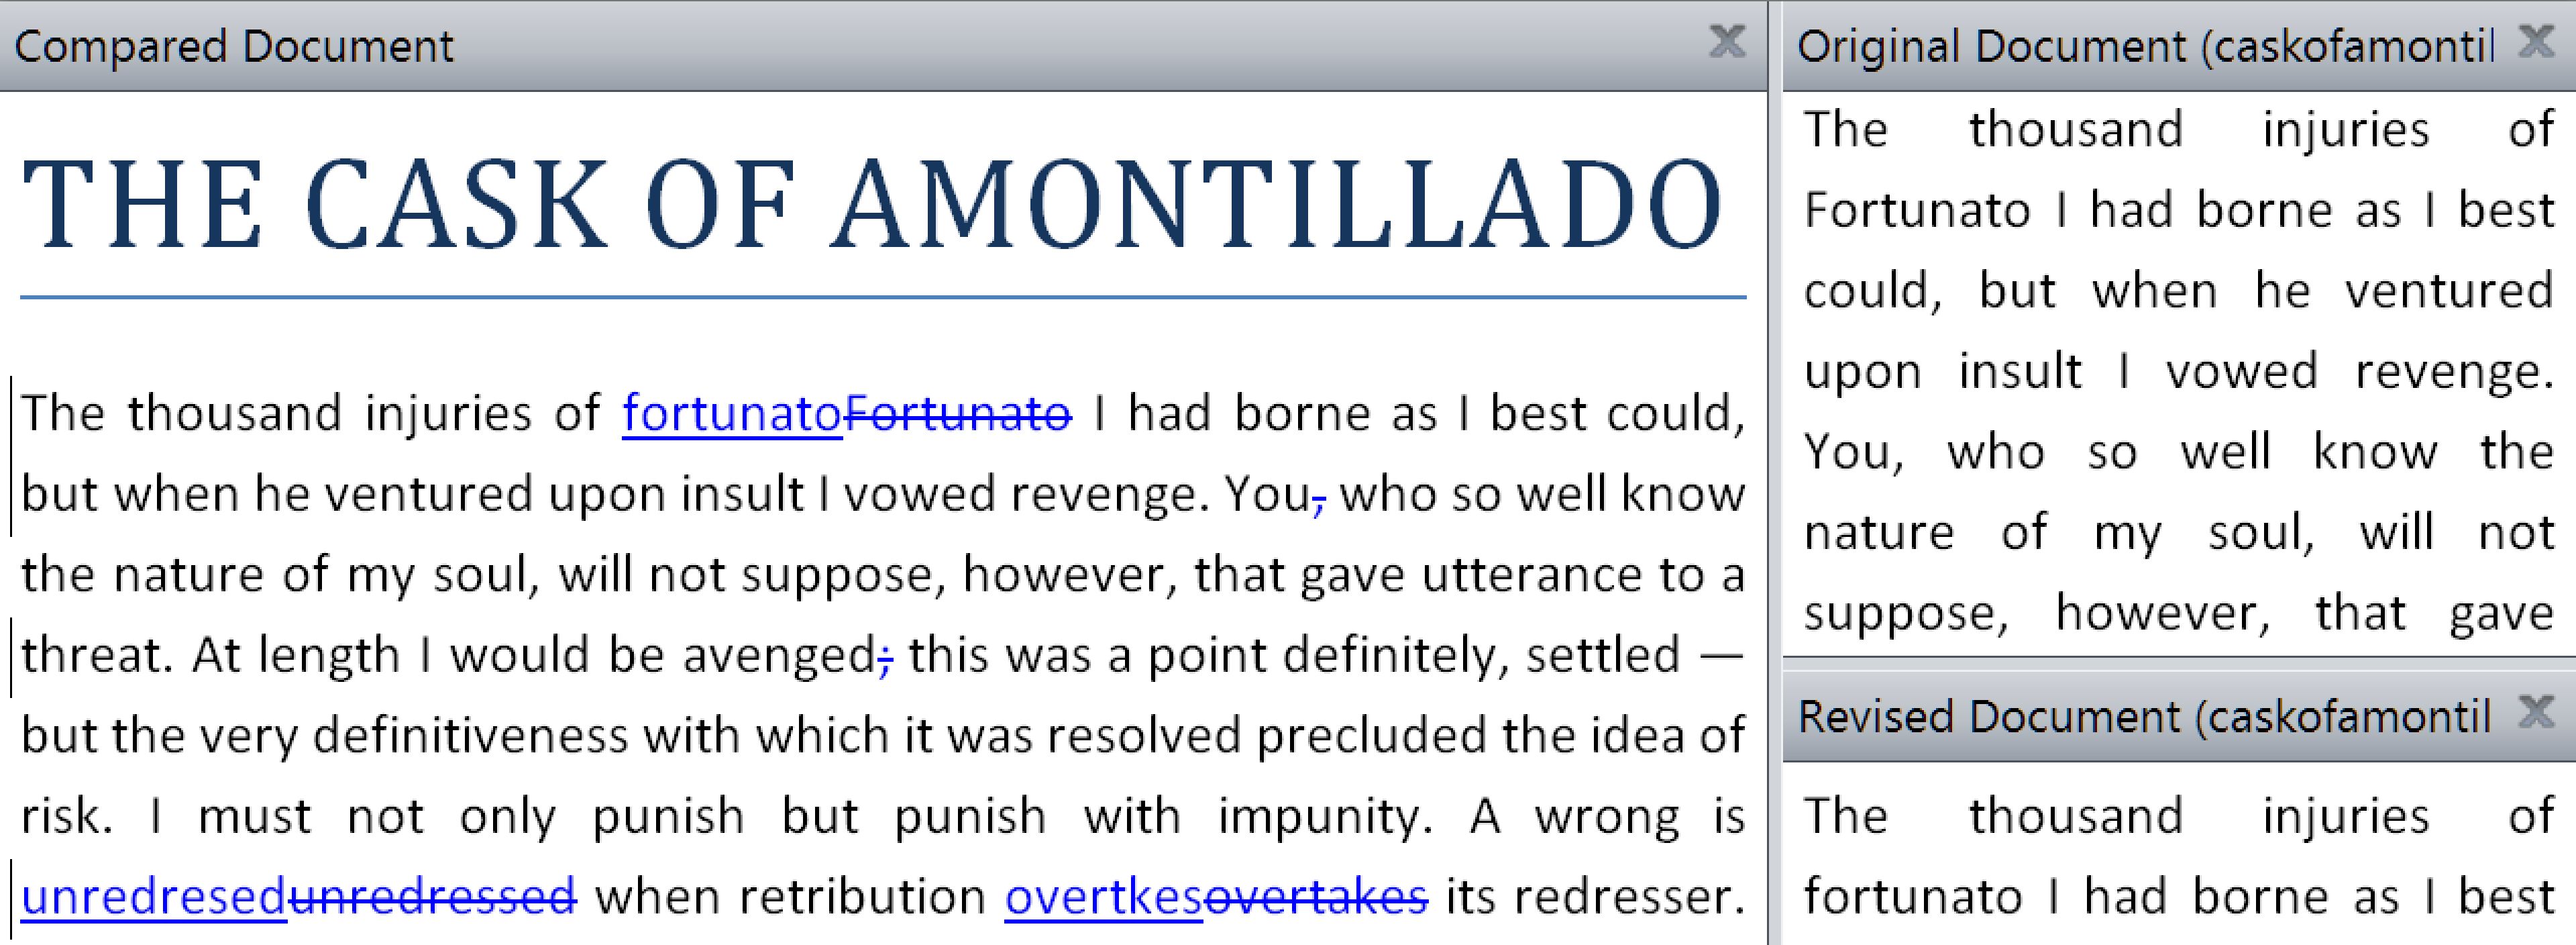
\includegraphics[width=\textwidth]{examples/01/tortoise-svn.png}
  \caption{\inx{Tortoise \acroshort{SVN}} is a graphical frontend for
    \acronym{SVN} with the ability to display the difference between two versions
    of a \inx{Microsoft Word} document even though it is not a text file.}
\end{figure}

%%% Git porcelains <http://stackoverflow.com/a/6978402>
%%% Git <-> SVN
%%%   <https://git-scm.com/book/en/v1/Git-and-Other-Systems-Git-and-Subversion>
%%%   <http://www.janosgyerik.com/practical-tips-for-using-git-with-large-subversion-repositories/>
%%%   <http://stackoverflow.com/a/772881/657401>
